% Journal draft for IEEE Access. Written in IEEEtran (journal) so it compiles anywhere; move the
% body into the official IEEE Access template (ieeeaccess.cls, on Overleaf) at submission.
% Every number in tables/ and in the theory section is generated by jr/tables.py from the result
% files; the numbers in the running text are checked by jr/paper_checks.py.
\documentclass[journal]{IEEEtran}
\usepackage{amsmath,amssymb,amsthm}
\usepackage{booktabs}
\usepackage{multirow}
\usepackage{cite}
\usepackage{url}
\usepackage{graphicx}
\newtheorem{proposition}{Proposition}
\newtheorem{definition}{Definition}
\newcommand{\PiZero}{0.867}
\newcommand{\NegAll}{496}
\newcommand{\NegStruct}{430}
\newcommand{\AucNonempty}{0.885}
\newcommand{\AucAll}{0.985}
\newcommand{\AucPred}{0.985}
\newcommand{\AZero}{1.000}
\newcommand{\Inflation}{0.099}
\newcommand{\TrainPrev}{0.41}
\newcommand{\TrainRatio}{1.4}
\newcommand{\ExtProjects}{8}
\newcommand{\PrevMin}{0.07}
\newcommand{\PrevMax}{0.59}
\newcommand{\RatioMin}{13}
\newcommand{\RatioMax}{0.7}
\newcommand{\SensMin}{0.00}
\newcommand{\SensMax}{0.86}
\newcommand{\SpearmanPS}{0.93}
\newcommand{\CarryMedian}{0.67}
\newcommand{\Qhat}{0.33}
\newcommand{\PSpillThree}{0.963}
\newcommand{\NonemptySpill}{90.1}
\newcommand{\MedianIssues}{6}
\newcommand{\OverlapShare}{57}
\newcommand{\NoFallbackTest}{356}
\newcommand{\FallbackMean}{12.9}
\newcommand{\Rhat}{0.18}
\newcommand{\DispRatio}{4.5}
\newcommand{\LRstat}{2,181}

% \input is not expandable inside tabular in current LaTeX; the primitive is.
\makeatletter\newcommand{\tabinput}[1]{\@@input #1 }\makeatother

\begin{document}

\title{Predicting Sprint Trouble Without Hindsight: A Benchmark of Feature Families on 29 Public Jira Projects}

% Co-authors to be confirmed before submission.
\author{Hani~AbuSharkh%
\thanks{H. AbuSharkh is with the Higher Colleges of Technology, Al Ain, UAE (e-mail: habusharkh@hct.ac.ae).}}

\maketitle

\begin{abstract}
Sprint-risk models are usually built from a present-day Jira export, which shows how a sprint ended rather than what the team knew when it began. Studies also report their own features on their own data, so it is not known which kinds of signal actually carry the prediction. We address both problems. We state formally what a feature may use at prediction time and derive three consequences: empty sprints inflate ROC-AUC by a computable amount, a threshold fitted on one group of teams implies a cost ratio that does not hold for another, and a simple binomial model says which spillover label history should help with. We then score six feature families on the same 4,235 sprints from 29 TAWOS projects under one time-ordered protocol, with five outcomes: late closure and spillover, and three labels new to this study (serious spillover, seriously late, scope churn). Progress counts dominate during the sprint. Burndown-shape features, built after a recent study, add nothing on top of progress counts and, for lateness early in the sprint, rank worse than committed scope alone. Planning-time team history adds about 0.05 to 0.07 AUC on top of progress counts for the spillover labels. Four new planning-time features add about 0.03 AUC for spillover and serious spillover and nothing for lateness. Serious spillover is the most useful new label: history beats scope by 0.10 AUC, as the binomial model predicts, although our own pre-stated hypothesis said the opposite. On ten outside projects from MariaDB and MongoDB, none of the history gains transfer.
\end{abstract}

\begin{IEEEkeywords}
Agile software development, data leakage, Jira, machine learning, mining software repositories, Scrum, sprint risk, ROC analysis
\end{IEEEkeywords}

\section{Introduction}

\IEEEPARstart{A}{} Scrum team commits to a set of issues at the start of each sprint. Some sprints end with work left over, and some are closed in Jira days after their planned end. Both are visible to everyone once the sprint is over. The useful question is whether they can be seen coming, at planning or early in the sprint, from what the tracker already records.

Several studies have tried \cite{choet2018,sprint2vec,hearty2009,perez2024,obike2025}. Two things make their results hard to use. The first is hindsight. A Jira export is a snapshot taken years later: an issue's sprint field, story points and status are the final values unless the change log is replayed. A model trained on the snapshot can learn from facts that did not exist at planning, and its accuracy then says little about what a team would see in practice \cite{kaufman2012,kapoor2023}. The second is that every study brings its own features, labels, data and protocol. If one paper reports a good AUC with burndown features and another with iteration counts, nobody can tell which kind of signal does the work, because the two numbers were never measured on the same sprints.

This paper takes both problems in turn. Our earlier work \cite{abusharkh2027} rebuilt the board as it stood on the first day of each sprint for eight TAWOS projects \cite{tawos}, and showed how much two common mistakes inflate the results. Here we turn the same reconstruction into a benchmark. We extend it to every TAWOS project with enough sprints (29 projects, 4,235 sprints), state the no-hindsight rule formally, and score six feature families side by side on the same sprints, the same labels and the same split.

The contributions are as follows.
\begin{enumerate}
\item \emph{A formal setting with checkable consequences} (Section~\ref{sec:theory}). We define an admissible feature as one that depends only on events logged before the prediction time, and derive three results: an exact decomposition of how empty sprints inflate ROC-AUC, the cost ratio a Youden threshold silently assumes, and a binomial model that says which spillover label history should help with. Each result is checked against our data.
\item \emph{A head-to-head benchmark} (Sections~\ref{sec:setup} to \ref{sec:results}). Committed scope, planning-time team history, four new planning-time features, in-sprint progress counts, burndown-shape features after P\'erez Castillo et al.\ \cite{perez2024}, and the iteration features of Choetkiertikul et al.\ \cite{choet2018} that a public export supports, all scored under one protocol with one stated primary analysis and two kinds of bootstrap interval.
\item \emph{Three new outcome labels with a verdict on each}: serious spillover, seriously late and scope churn. We report which ones a model can rank and which ones look like team habit.
\item \emph{An outside test} on ten projects from two organisations that are not in TAWOS, which shows where the gains stop.
\end{enumerate}

The short answer is that progress counts carry most of the in-sprint signal, burndown shape adds nothing, team history helps with how much is left over but not with when the sprint closes, and none of the history gains survive a move to another organisation. We wrote our hypotheses down before the full run (Section~\ref{sec:protocol}) and report where they failed. One failed in an instructive way: we expected history to add nothing to serious spillover, and the theory in Section~\ref{sec:theory} predicted the opposite. The theory was right.

\section{Related Work}
\label{sec:related}

\subsection{Predicting iteration outcomes}

Choetkiertikul et al.\ \cite{choet2018} predicted how much of an iteration's committed work would be delivered, using iteration-level counts (issues and points at start, added, removed, done, to do) together with issue-level and team features, on five open-source projects. Sprint2Vec \cite{sprint2vec} learns a sprint embedding from issue text and developer activity. Hearty et al.\ \cite{hearty2009} modelled velocity in XP with a dynamic Bayesian network. More recently, P\'erez Castillo et al.\ \cite{perez2024} graded finished sprints from eleven burndown-shape indicators (R1 to R11) computed in their Worki tool, and Obike et al.\ \cite{obike2025} scored sprint deliverability with a weighted index. Effort estimation \cite{choet2019,porru2016,tawosi2023} is a neighbouring problem: it predicts the size of an issue, not the fate of a sprint.

These studies differ in data, labels and validation, and in how strictly features are limited to what was known at prediction time. In cross-validation over iterations, a training fold can hold iterations that happened after the test ones \cite{choet2018}. No study compares the feature families on common data. We do not claim to reproduce any of them. We implement the parts of two feature families that a public export supports and score them on our sprints, which measures the families, not the papers.

\subsection{Leakage and time-aware evaluation}

Leakage, where a model sees information it would not have when deployed, is a known cause of inflated results \cite{kaufman2012,kapoor2023}. In software analytics, random splits mix past and future \cite{bangash2020}, and labels that are only known later leak into features \cite{jimenez2019}. Predictive process monitoring \cite{teinemaa2019} faces the same problem with event logs and evaluates predictions at prefixes of a case. Alarm-based monitoring \cite{fahrenkrog2022} treats a warning as a decision with a cost, which is the view we take in Section~\ref{sec:theory}. Our earlier work \cite{abusharkh2027} showed, on eight TAWOS projects, that two reproduced leakage mistakes inflated F1 by up to 0.24 and that shuffling sprints before splitting added 0.07 AUC. The present paper reuses that reconstruction but none of its results.

% Formal setting. Every number here comes from tables/numbers.tex, written by jr/tables.py
% from results/<cohort>/theory_numbers.json, and is checked by jr/theory_checks.py.

\section{Formal Setting}
\label{sec:theory}

This section fixes what ``no hindsight'' means for a Jira export and derives three consequences. Each one turns a pattern that is easy to miss into a prediction the experiments can check: how empty sprints inflate ROC-AUC, why a threshold fitted on one group of teams does not carry to another, and how the two spillover labels should differ.

\subsection{The event log and the sprint state}

A Jira export is an event log $\mathcal{E} = \{(i, f, v^{-}, v^{+}, t)\}$: issue $i$ had field $f$ changed from $v^{-}$ to $v^{+}$ at time $t$. With each issue's creation time $\gamma_i$ and resolution time $r_i$ (undefined while the issue is open), the log gives the value of any field at any time by replaying the changes in order. Write $\mathcal{E}_{\le t}$ for the events up to time $t$, and $\mathcal{F}_t$ for what they tell us together with the sprint calendar, which is fixed at planning. A sprint $s$ has a start $a_s$, a planned end $b_s$ and a closure time $c_s$.

The committed set is the board at the start,
\begin{equation}
C_s = \{\, i : s \in \mathrm{sprint}_i(a_s),\ \gamma_i \le a_s,\ r_i \not< a_s \,\},
\label{eq:committed}
\end{equation}
where $\mathrm{sprint}_i(t)$ is the issue's sprint field at time $t$ as replayed from $\mathcal{E}_{\le t}$. The outcomes are read off the end state. With $n_s = |C_s|$ and the carry ratio
\begin{equation}
\rho_s = \frac{|\{ i \in C_s : r_i > b_s \}|}{n_s},
\end{equation}
spillover is $y^{\mathrm{sp}}_s = \mathbf{1}[\rho_s > 0]$, serious spillover is $y^{\tau}_s = \mathbf{1}[\rho_s \ge \tau]$, late closure is $y^{\mathrm{late}}_s = \mathbf{1}[c_s - b_s > \delta]$ with $\delta$ one day (three for ``seriously late''), and scope churn is $\mathbf{1}[m_s / n_s \ge \theta]$, where $m_s$ counts issues added after $a_s$ and still in the sprint at $b_s$.

\subsection{Admissible features}

\begin{definition}[Admissible feature]
A feature $x(s, t)$ for sprint $s$ at prediction time $t$ is admissible if it is a function of $\mathcal{F}_t$ alone, that is, of $\mathcal{E}_{\le t}$ and the sprint calendar.
\end{definition}

Two common practices break this rule. First, a history feature that summarises an earlier sprint $u$ of the same project is admissible at $a_s$ only if $u$'s outcome was known by then, $\max(b_u, c_u) \le a_s$. A ``previous sprint'' picked by start date alone breaks this whenever sprints overlap, which happens for \OverlapShare\% of the sprints in our cohort. Second, a field read from the static export is $\mathcal{F}_\infty$-measurable, not $\mathcal{F}_{a_s}$-measurable. Wherever the log records no change for a field, the replay has to fall back on a value that may postdate planning. We record the share of committed issues affected, $\phi_s$, and repeat the main comparisons on sprints with $\phi_s = 0$. Issue type, priority and assignee are left out altogether, because the export only holds their final values.

\subsection{Empty sprints inflate ROC-AUC}

A sprint with $n_s = 0$ cannot spill, so it is a negative by construction. Keeping such sprints in a spillover evaluation rewards the model for something it did not have to learn.

\begin{proposition}
\label{prop:auc}
Split the negatives of a test set into structural negatives $N_0$ and ordinary negatives $N_1$, and let $\pi_0 = |N_0| / (|N_0| + |N_1|)$. Then
\begin{equation}
\mathrm{AUC}_{\mathrm{all}} = \pi_0\, A_0 + (1 - \pi_0)\, \mathrm{AUC}_{N_1},
\label{eq:aucmix}
\end{equation}
where $A_0$ is the probability that a random positive outscores a random structural negative, and $\mathrm{AUC}_{N_1}$ is the AUC on the positives and ordinary negatives alone. If the model ranks every structural negative below every positive, $A_0 = 1$ and the inflation is $\pi_0 (1 - \mathrm{AUC}_{N_1})$.
\end{proposition}

\begin{proof}
AUC is the probability that a random positive outscores a random negative. Conditioning on which kind of negative is drawn gives (\ref{eq:aucmix}).
\end{proof}

The decomposition is elementary. Its use is that it puts an exact number on the inflation.

On our time-split test set the full population has \NegAll{} negatives, and \NegStruct{} of them commit nothing, so $\pi_0 = \PiZero$. The model's AUC on nonempty sprints is \AucNonempty. With $A_0 = 1$, (\ref{eq:aucmix}) predicts \AucPred{} for the full population; the observed value is \AucAll, and the measured $A_0$ is \AZero. The gap of \Inflation{} between the two headline numbers is entirely the empty sprints. Any study that keeps them in the denominator reports this gap as skill.

\subsection{Why a fitted threshold does not travel}

Youden's index picks the threshold that maximises sensitivity plus specificity, which is the same as minimising $\mathrm{FNR} + \mathrm{FPR}$. With prevalence $\pi$, a miss cost $c_{\mathrm{FN}}$ and a false-alarm cost $c_{\mathrm{FP}}$, the expected cost per sprint is $\pi c_{\mathrm{FN}} \mathrm{FNR} + (1 - \pi) c_{\mathrm{FP}} \mathrm{FPR}$. This is proportional to $\mathrm{FNR} + \mathrm{FPR}$ exactly when
\begin{equation}
\frac{c_{\mathrm{FN}}}{c_{\mathrm{FP}}} = \frac{1 - \pi}{\pi}.
\label{eq:youden}
\end{equation}

\begin{proposition}
\label{prop:youden}
A Youden threshold fitted on a population with prevalence $\pi_{\mathrm{train}}$ is cost-optimal on a population with prevalence $\pi$ only if the implied cost ratio (\ref{eq:youden}) is the same, that is, only if $\pi = \pi_{\mathrm{train}}$. For a calibrated score the cost-optimal rule warns when $p \ge p^{*} = c_{\mathrm{FP}} / (c_{\mathrm{FP}} + c_{\mathrm{FN}})$, which does not depend on prevalence. A fixed score threshold carried to a team with lower prevalence therefore acts like a rule that prices a miss at only $(1 - \pi_{\mathrm{train}}) / \pi_{\mathrm{train}}$ false alarms, and its sensitivity falls with $\pi$.
\end{proposition}

The link between a threshold rule and the cost ratio it implies is standard in the ROC literature \cite{hernandez2012}. What we add is its use to explain why a threshold that worked on TAWOS misses most failures on some new teams.

For late closure the training prevalence is \TrainPrev, so the implied ratio is \TrainRatio. On the \ExtProjects{} testable outside projects the same threshold meets prevalences from \PrevMin{} to \PrevMax, where (\ref{eq:youden}) would call for ratios from \RatioMin{} down to \RatioMax. The observed sensitivity runs from \SensMin{} to \SensMax, with a rank correlation of \SpearmanPS{} with prevalence. The ranking travels because AUC does not depend on a threshold; the threshold does not travel. A deployment has to recalibrate it per team or set it from stated costs.

\subsection{A minimal model of the two spillover labels}

Suppose each committed issue of sprint $s$ is finished by the planned end independently with probability $q_s$, a property of the team and the period rather than of the issue. The number left unfinished is then $\mathrm{Binomial}(n_s, 1 - q_s)$, and
\begin{align}
\Pr[y^{\mathrm{sp}}_s = 1] &= 1 - q_s^{\,n_s}, \label{eq:any}\\
\mathbb{E}[\rho_s] &= 1 - q_s, \qquad \mathrm{Var}[\rho_s] = \frac{q_s (1 - q_s)}{n_s}. \label{eq:ratio}
\end{align}
Two predictions follow. By (\ref{eq:any}) the ``any'' label is driven by $n_s$ and saturates fast: at the cohort's median carry ratio, \CarryMedian, $q_s \approx \Qhat$ and a sprint of three issues already spills with probability \PSpillThree. The median nonempty sprint commits \MedianIssues{} issues, and \NonemptySpill\% of nonempty sprints spill. So committed scope should carry most of what can be known about plain spillover. By (\ref{eq:ratio}) a threshold label on $\rho_s$ is driven by $1 - q_s$, the team's completion rate, with $n_s$ entering only through the variance. Serious spillover should therefore depend on planning-time history and capacity rather than on scope, and the gap between scope-only and history-aware models should be larger for it than for plain spillover. Section~\ref{sec:results} tests both. The model ignores dependence between issues and scope changes during the sprint. It is a reading aid, not a claim about how teams work.

\subsection{Warnings as decisions}

A warning raised at checkpoint $c$ costs $\kappa$ and, if the sprint would otherwise fail, averts a fraction $e(c)$ of the failure cost $F$, with $e$ falling as $c$ grows. Warning at calibrated risk $p$ has expected cost $\kappa + F p (1 - e(c))$ against $F p$ for staying silent, so the warning pays when
\begin{equation}
p \ge \frac{\kappa}{e(c)\, F}.
\label{eq:warn}
\end{equation}
The bar rises as the sprint goes on, because a late warning saves less. An in-sprint model is useful only where its gain in ranking outpaces the fall in $e(c)$. Because (\ref{eq:warn}) needs a calibrated $p$, we report calibration beside AUC.


\section{Data and Reconstruction}
\label{sec:setup}

\subsection{Cohort}

TAWOS \cite{tawos} holds Jira data from open-source projects; 36 of them have sprints. We count a sprint as usable if it is closed, has start, end and completion dates, and neither the end nor the completion is before the start. Thirty-two projects have at least 30 usable sprints. Three of them (MongoDB Compass and the MongoDB C++ and Java drivers) are also in our outside test set, which we pulled from MongoDB's live Jira, so we drop them from TAWOS to keep the outside test clean. The cohort is the remaining 29 projects. After dropping each project's first sprint as a cold start, it has 4,235 sprints from February 2012 to October 2020, between 35 and 557 per project (median 97). Of these, 2,671 commit at least one issue; we call them nonempty.

The outside set is the ten projects used in our earlier study: MariaDB MaxScale and ColumnStore, and eight MongoDB projects, exported from the organisations' public Jira and converted to the TAWOS layout. They are used only for testing.

\subsection{Reconstruction}

For every sprint we replay the Sprint and Story Points fields of every issue back to the sprint's start and form the committed set (\ref{eq:committed}). Issues added later, issues removed later, and their story points at the start all come from the replay. Where an issue has no recorded story-point change, the replay falls back on the exported value; on average \FallbackMean\% of a sprint's committed issues are affected. Two custom fields are excluded from the replay: ``Actual Story Points'' in Spring XD, which is recorded after the work, and a retired duplicate in Moodle. Code, queries and the exact export are in the repository listed under Data Availability.

\section{Outcomes, Features and Protocol}
\label{sec:protocol}

\subsection{Outcomes}

Table~\ref{tab:labels} lists the five outcomes. Late closure and spillover are carried over from our earlier work. The other three are new.

\emph{Serious spillover} asks how much was left over, not whether anything was. The primary threshold is a carry ratio of 30\%. The median nonempty sprint in TAWOS leaves 71\% of its committed issues unfinished, so this label is still 83\% positive. We therefore also report a median-based version (carry ratio above the training-set median, 52\% positive) and thresholds of 20\% and 50\%.

\emph{Seriously late} means the sprint was closed in Jira more than three days after its planned end (seven as a sensitivity check). Like late closure, it records an administrative event, only a larger one.

\emph{Scope churn} means the issues added after the start and still in the sprint at its planned end make up at least 30\% of the committed count (50\% as a sensitivity check). It is defined only for sprints with five or more committed issues, because one added issue in a two-issue sprint is 50\%. It is predicted at planning time only, because during the sprint the additions so far give the answer away.

\begin{table}[t]
\centering
\small
\caption{Outcomes, populations and positive rates (29 TAWOS projects). Nonempty: sprints that commit at least one issue. Indented rows are sensitivity versions.}
\label{tab:labels}
\begin{tabular}{@{}llrr@{}}
\toprule
Outcome & Population & Sprints & Positive \\
\midrule
\tabinput{tables/labels.tex}
\bottomrule
\end{tabular}
\end{table}

\subsection{Feature families}

Table~\ref{tab:families} lists the six families. All features are admissible in the sense of Section~\ref{sec:theory}.

\begin{table}[t]
\centering
\small
\caption{Feature sets. Planning-time sets are scored at the sprint start; in-sprint sets at 25\% and 50\% of the planned duration.}
\label{tab:families}
\begin{tabular}{@{}p{1.6cm}p{6.3cm}@{}}
\toprule
Set & Contents \\
\midrule
scope & Committed issues, committed story points, sprint length. \\
strict & scope, parallel sprints, the last three finished sprints (completion ratio, carry-over, delivered points, completed and committed issues), scope relative to capacity, past lateness, and the project. \\
strict+new & strict and the four new features below. \\
choet & Iteration features of \cite{choet2018} that the export supports: duration, issues and points at start, added and removed since start, done and to do at the checkpoint. \\
worki & Burndown-shape indicators R1 to R11 after \cite{perez2024}, on issue counts. \\
ours & strict+new and 13 progress counts: elapsed share, days left, done and remaining issues and points, burn gap, required and observed rate, added and removed ratios. \\
ours+worki & ours and R1 to R11. \\
\bottomrule
\end{tabular}
\end{table}

The four \emph{new planning-time features} are: the share of committed issues that had been in another sprint before (carried in); the log of the median age of committed issues at the start; the share of committed issues with no estimate; and the share whose estimate was changed before the start (re-estimated). Each is computed from the replayed log.

The \emph{worki} set follows our reading of the verbal definitions in \cite{perez2024}, computed on the daily burndown of issue counts up to the checkpoint. Their study graded finished sprints; we score the same kind of indicator during the sprint, which is a different task. The \emph{choet} set leaves out what a public export cannot support: in-progress counts (there is no status history), team size and the Scrum master (the assignee is a final value), and all issue-level features. At planning time their supported set reduces to our scope set. Neither comparison therefore ranks the two studies; each measures a family of signal.

One asymmetry matters for reading the results. The strict and ours sets include the project as a categorical feature, as in our earlier work; scope, choet and worki do not. On the time split, part of a strict or ours gain may therefore be project identity. Leave-one-project-out testing removes the project from every set, and we report it beside every primary result.

\subsection{Models and protocol}

We use logistic regression with balanced class weights, a random forest (300 trees, depth 5) and histogram gradient boosting (depth 3, learning rate 0.05, 200 iterations), all from scikit-learn \cite{sklearn} with fixed settings and seed 42. There is no hyperparameter search.

The \emph{primary analysis} is gradient boosting on a per-project time split: the first 70\% of each project's sprints by start date for training, the rest for testing (1,288 test sprints, 814 of them nonempty). For each outcome and each comparison we report one paired AUC difference with two 95\% bootstrap intervals from 2,000 resamples: one that resamples whole projects, which is the test, and one that resamples sprints, which is reported beside it. Everything else is secondary and read as a pattern: the other two models, leave-one-project-out testing, five time-ordered repeats (training on the first 40\% to 80\% of each project and testing on the next 20\%), and the outside projects (trained on all of TAWOS, without the project feature and without story points, which MariaDB does not record). Decision thresholds are fixed by Youden's index on out-of-fold training scores, never on the test set.

\subsection{Hypotheses}

We wrote the study plan, the primary analysis and four hypotheses into a dated plan before the full-cohort run, and logged every later change with its reason. A hypothesis holds only where the project-level interval is above zero.
\begin{itemize}
\item \textbf{H1} (new features, strict+new minus strict, planning time): positive for scope churn and serious spillover, small and positive for spillover, about zero for the two late labels.
\item \textbf{H2} (burndown shape, ours minus worki, spillover labels): positive at both checkpoints.
\item \textbf{H3} (planning context on top of progress counts, ours minus choet): positive and below 0.05 for every outcome.
\item \textbf{H4} (new labels can be ranked, strict+new minus scope): positive for seriously late and scope churn, about zero for serious spillover.
\end{itemize}
The plan was written after a development run on eight of the 29 projects, which are part of the final cohort. Section~\ref{sec:threats} discusses what that means.

\section{Results}
\label{sec:results}

\subsection{Planning time}

Table~\ref{tab:planauc} gives the AUC of the three planning-time sets and Table~\ref{tab:planprimary} the primary differences.

\begin{table}[t]
\centering
\small
\caption{Planning-time ROC-AUC, gradient boosting. Time: per-project time split. LOPO: leave one project out (no project feature).}
\label{tab:planauc}
\setlength{\tabcolsep}{4pt}
\begin{tabular}{@{}lrrrrrr@{}}
\toprule
& \multicolumn{3}{c}{Time split} & \multicolumn{3}{c}{LOPO} \\
\cmidrule(lr){2-4}\cmidrule(l){5-7}
Outcome & scope & strict & +new & scope & strict & +new \\
\midrule
\tabinput{tables/planning_auc.tex}
\bottomrule
\end{tabular}
\end{table}

\begin{table}[t]
\centering
\footnotesize
\caption{Primary planning-time differences in AUC (gradient boosting, time split) with 95\% bootstrap intervals over projects and over sprints. H1: strict+new minus strict. H4: strict+new minus scope.}
\label{tab:planprimary}
\setlength{\tabcolsep}{3.5pt}
\begin{tabular}{@{}llrcc@{}}
\toprule
& Outcome & $\Delta$ & Projects & Sprints \\
\midrule
\tabinput{tables/primary_planning.tex}
\bottomrule
\end{tabular}
\end{table}

\emph{H1 holds for the two spillover labels.} The new features add 0.028 [0.007, 0.047] for spillover and 0.026 [0.004, 0.050] for serious spillover. The gain has the same sign for all three models and under leave-one-project-out testing (0.020 [0.006, 0.037] and 0.027 [0.009, 0.048]). For the two late labels the difference is about zero, as predicted. For scope churn it is 0.042, but the project interval just crosses zero, so H1 does not hold there.

\emph{H4 fails where it was most specific.} We predicted that history would add nothing to serious spillover beyond scope. It adds 0.104 [0.036, 0.179] on the time split and 0.168 [0.111, 0.223] under leave-one-project-out testing, the largest planning-time gain in the study. Seriously late (0.033) and scope churn (0.088) are positive on the sprint-level interval only, so H4 does not hold for either.

\emph{Late closure is hard.} Scope alone reaches 0.718, and nothing at planning time does much better.

\subsection{The binomial model's prediction}

Section~\ref{sec:theory} predicts that history should beat scope by more for serious spillover than for plain spillover. It does. On the time split, strict minus scope is 0.012 for spillover against 0.079 for serious spillover; under leave-one-project-out testing it is 0.032 against 0.141. Plain spillover is mostly a matter of how many issues were committed, and serious spillover is mostly a matter of which team committed them. The prediction contradicts H4, which we wrote on the same day; the data side with the model.

\subsection{During the sprint}

Tables~\ref{tab:inauc} and \ref{tab:inprimary} give the in-sprint results. All sets are scored on the nonempty sprints still open at the checkpoint (810 test sprints at 25\%, 803 at 50\%), so late closure here has a different population from Table~\ref{tab:planauc}.

\begin{table}[t]
\centering
\small
\caption{In-sprint ROC-AUC at 25\% and 50\% of the planned duration, gradient boosting, time split.}
\label{tab:inauc}
\setlength{\tabcolsep}{3.5pt}
\begin{tabular}{@{}llrrrrr@{}}
\toprule
Outcome & At & scope & worki & choet & ours & +worki \\
\midrule
\tabinput{tables/insprint_auc.tex}
\bottomrule
\end{tabular}
\end{table}

\begin{table*}[t]
\centering
\caption{Primary in-sprint differences in AUC (gradient boosting, time split) with 95\% bootstrap intervals over projects and over sprints. The worki minus scope rows are not a hypothesis and are given for reading.}
\label{tab:inprimary}
\begin{tabular}{@{}lllrrcc@{}}
\toprule
& Comparison & Outcome & At & $\Delta$ & Projects & Sprints \\
\midrule
\tabinput{tables/primary_insprint.tex}
\bottomrule
\end{tabular}
\end{table*}

\emph{H2 holds.} Our set beats the burndown-shape set by 0.118 to 0.223 AUC on both spillover labels at both checkpoints. The burndown set is not just weaker than ours. For late closure at 25\%, for seriously late at both checkpoints and for spillover at 50\%, it ranks worse than committed scope alone, with intervals below zero, and adding it to our set changes nothing (every ours+worki minus ours difference is within 0.012).

\emph{H3 holds in direction, not in size.} Planning context adds to progress counts for every outcome, and the project interval clears zero for both spillover labels (0.046 to 0.067). For serious spillover the gain is above the 0.05 we expected. Because ours includes the project feature and choet does not, we checked the same comparison under leave-one-project-out testing, where neither set has it: the gain stays at 0.036 [0.012, 0.065] and 0.028 [0.008, 0.052] for spillover, and 0.078 [0.053, 0.106] and 0.064 [0.039, 0.092] for serious spillover. For the two late labels the project intervals include zero.

\emph{The spillover labels are where the signal is.} Serious spillover goes from 0.775 at planning time to 0.851 at 25\% and 0.891 at 50\%. For late closure our set reaches only 0.718 and 0.722, against 0.687 and 0.682 for scope alone on the same sprints.

\subsection{Outside projects}

Table~\ref{tab:external} trains on all of TAWOS and tests on each outside project with at least five sprints in each class. Nothing transfers reliably. For the two spillover labels, where history helped most inside TAWOS, it does not help outside: scope alone scores 0.785 for spillover and 0.592 for serious spillover, and the history-aware sets score lower. For late closure all three sets sit near 0.65. The spread across projects is about $\pm 0.1$ to $\pm 0.2$. This fits the reading in Section~\ref{sec:theory}: history features estimate one team's completion rate, and that estimate does not carry to another organisation's teams.

\begin{table}[t]
\centering
\footnotesize
\caption{Outside projects: mean $\pm$ s.d.\ of per-project AUC, gradient boosting trained on all TAWOS sprints. $k$: projects with at least five sprints in each class.}
\label{tab:external}
\setlength{\tabcolsep}{3pt}
\begin{tabular}{@{}lrccc@{}}
\toprule
Outcome & $k$ & scope & strict & strict+new \\
\midrule
\tabinput{tables/external.tex}
\bottomrule
\end{tabular}
\end{table}

\subsection{Calibration and decisions}

Table~\ref{tab:calibration} gives the Brier score, the Brier score of always predicting the test prevalence, the expected calibration error over ten bins, and the calibration slope. For the spillover labels the models are well calibrated (slopes 0.88 to 1.04) and clearly beat the reference. For the late labels they are overconfident (slopes 0.55 to 0.85), and for seriously late during the sprint the Brier score is no better than the reference. By (\ref{eq:warn}), an in-sprint lateness warning built on these scores would rest on probabilities that are not trustworthy.

\begin{table}[t]
\centering
\small
\caption{Calibration on the time-split test set, gradient boosting. Ref.: Brier score of the test prevalence. ECE: expected calibration error, ten bins.}
\label{tab:calibration}
\setlength{\tabcolsep}{3.5pt}
\begin{tabular}{@{}llrrrr@{}}
\toprule
Outcome & Stage & Brier & Ref. & ECE & Slope \\
\midrule
\tabinput{tables/calibration.tex}
\bottomrule
\end{tabular}
\end{table}

With a Youden threshold from the training folds, the planning-time model flags serious spillover with sensitivity 0.73 at specificity 0.69, spillover with 0.68 at 0.85, and late closure with 0.62 at 0.76.

\subsection{Further checks}

\emph{Provenance.} On the \NoFallbackTest{} nonempty test sprints with no story-point fallback, the new features add 0.023 [$-$0.007, 0.051] for spillover and 0.027 [$-$0.001, 0.053] for serious spillover: the same size as the primary result, with intervals that just touch zero. The gain is not an artefact of fallback values, but this subset alone would not establish it.

\emph{Other thresholds.} The median-based serious-spillover label behaves like the primary one: strict+new scores 0.720 against 0.572 for scope, and the new features add 0.032 [0.007, 0.056]. At the 50\% threshold they add 0.032 [0.006, 0.061] and at 20\% 0.036 [0.019, 0.064]. For scope churn at 50\% they add 0.054 [0.015, 0.087], so the primary scope-churn result may be a near miss rather than a null.

\emph{Repeats.} The five time-ordered repeats agree with the time split: strict+new scores 0.860 $\pm$ 0.016 for spillover, 0.769 $\pm$ 0.022 for serious spillover and 0.728 $\pm$ 0.013 for late closure.

\subsection{Summary of hypotheses}

\begin{figure}[t]
\centering
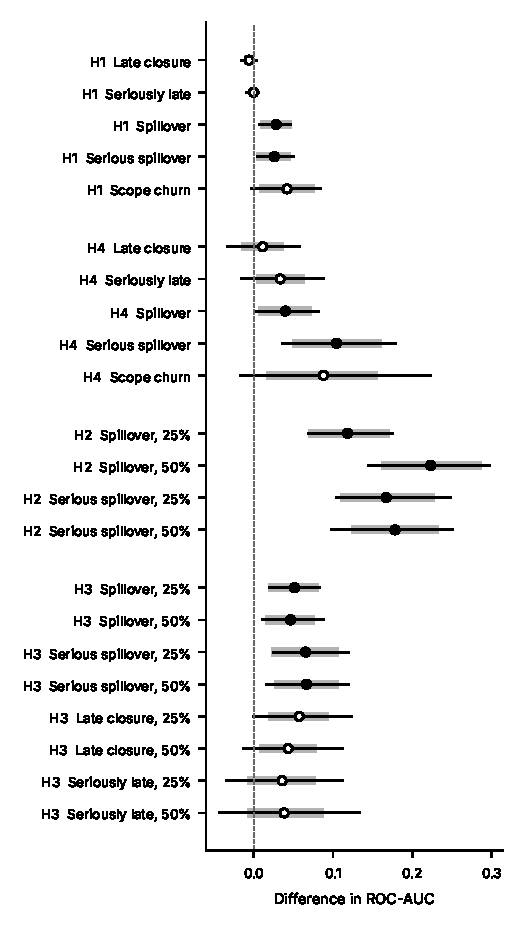
\includegraphics[width=\columnwidth]{fig_primary.pdf}
\caption{Every hypothesis comparison in the primary analysis. Dot: difference in AUC (filled where the project-level interval is above zero, the rule for a hypothesis to hold). Black line: 95\% interval over projects. Grey bar: 95\% interval over sprints.}
\label{fig:primary}
\end{figure}

Fig.~\ref{fig:primary} puts all 22 comparisons on one scale. H1 holds for spillover and serious spillover and is about zero for lateness, as predicted, but misses for scope churn. H2 holds. H3 holds in direction for every outcome and clears zero for the spillover labels, with a larger gain than predicted for serious spillover. H4 fails: serious spillover, predicted to be unrankable beyond scope, gives the largest gain, and the other two new labels pass only on the sprint-level interval.

\section{Discussion}
\label{sec:discussion}

\subsection{What a team can take from this}

Three things. First, during a sprint, simple progress counts (how much is done, how much is left, how fast it is going) carry nearly all of the signal, and their warnings for leftover work are calibrated. Burndown-shape indicators add nothing on top of them and, for lateness, do worse than knowing the sprint's size. Second, before a sprint starts, the team's own recent history is what says how much will be left over, and the four new features add a little to it. Third, none of this travels. A model trained on other organisations' teams is no better than a size rule, and a threshold carried from one team to another changes what a miss is worth (Proposition~\ref{prop:youden}). A team that wants these warnings has to fit them on its own history.

\subsection{Why lateness is hard}

Late closure is the moment someone pressed ``Complete sprint'' in Jira. That depends on meetings, holidays and habit as much as on the work, and no feature family we tried moves it much. We keep it for continuity, but we would not build a tool on it. Seriously late, the larger version of the same event, is no easier to rank, and its scores are the worst calibrated in the study.

\subsection{Threats to validity}
\label{sec:threats}

\emph{Construct.} The labels come from Jira fields, not from asking teams whether a sprint went badly. Late closure and seriously late measure when a sprint was closed in the tool. Spillover counts issues, not effort.

\emph{Internal.} The reconstruction depends on the change log. Where it is missing, story points fall back on the exported value; we measured the share and repeated the main comparisons without it. Issue type, priority and assignee are left out because only their final values exist, which also means the choet set lacks team and issue features that its authors used. The strict and ours sets carry the project as a feature; we repeated the main comparisons without it.

\emph{Hypotheses written after a look at the data.} The plan, the primary analysis and the hypotheses were written before the full run but after a development run on eight of the 29 projects, which hold 2,602 of the 4,235 sprints. Some choices were made after that look, most clearly the median-based serious-spillover label, and all of them are logged with dates. The hypotheses are therefore not independent of 8 of the 29 projects. Two things limit the damage: the hypotheses that failed (H4, the size in H3) failed against what the development run had suggested, and the outside projects were never used for any decision.

\emph{Conclusion.} The four hypotheses rest on 22 paired comparisons with no correction for multiple testing. The project-level interval resamples 29 clusters, which is coarse; we report the sprint-level interval beside it and treat a result as holding only when the project interval clears zero.

\emph{External.} All projects are open source, and a handful of organisations (Atlassian, Appcelerator and a few others) contribute most TAWOS projects. The outside test covers two more organisations and ten projects, few of which have enough sprints in both classes for every label.

\section{Conclusion}

Under one leakage-aware protocol, the kinds of signal used in the sprint-risk literature differ sharply. Progress counts dominate during a sprint, burndown shape adds nothing, team history explains how much work is left over but not when the sprint is closed, and nothing learned from one organisation's history helps another's. The formal setting turns three of these observations into results that can be checked: empty sprints inflate AUC by an exact amount, a fitted threshold carries a hidden cost ratio, and the choice between ``any'' and ``serious'' spillover decides whether history can matter. The most useful outcome we added is serious spillover in its median-based form. The obvious next step is to ask teams whether the sprints these models flag are the ones they would have wanted to hear about.

\section*{Data Availability}

Code, export queries, the reconstructed frames, every result file and the dated study plan with its change log are at \url{https://github.com/hani-ziad/journal-ieee-access-2027}. TAWOS is available from its authors \cite{tawos}.

\begin{thebibliography}{99}

\bibitem{choet2018} M. Choetkiertikul, H. K. Dam, T. Tran, A. Ghose, and J. Grundy, ``Predicting delivery capability in iterative software development,'' \emph{IEEE Trans. Softw. Eng.}, vol. 44, no. 6, pp. 551--573, Jun. 2018.

\bibitem{sprint2vec} M. Choetkiertikul, P. Banyongrakkul, C. Ragkhitwetsagul, S. Tuarob, H. K. Dam, and T. Sunetnanta, ``Sprint2Vec: A deep characterization of sprints in iterative software development,'' \emph{IEEE Trans. Softw. Eng.}, vol. 51, no. 1, pp. 220--242, Jan. 2025.

\bibitem{hearty2009} P. Hearty, N. Fenton, D. Marquez, and M. Neil, ``Predicting project velocity in XP using a learning dynamic Bayesian network model,'' \emph{IEEE Trans. Softw. Eng.}, vol. 35, no. 1, pp. 124--137, Jan. 2009.

\bibitem{perez2024} Y. J. P\'erez Castillo, S. D. Orantes Jim\'enez, and P. O. Letelier Torres, ``Sprint management in Agile approach: Progress and velocity evaluation applying machine learning,'' \emph{Information}, vol. 15, no. 11, Art. no. 726, 2024.

\bibitem{obike2025} P. G. Obike, V. E. Ekong, and O. U. Obot, ``A novel scoring-based Agile sprint deliverability prediction and prioritization using machine learning,'' \emph{Int. J. Comput. Appl.}, vol. 187, no. 49, pp. 40--53, Oct. 2025.

\bibitem{kaufman2012} S. Kaufman, S. Rosset, C. Perlich, and O. Stitelman, ``Leakage in data mining: Formulation, detection, and avoidance,'' \emph{ACM Trans. Knowl. Discov. Data}, vol. 6, no. 4, Art. no. 15, 2012.

\bibitem{kapoor2023} S. Kapoor and A. Narayanan, ``Leakage and the reproducibility crisis in machine-learning-based science,'' \emph{Patterns}, vol. 4, no. 9, Art. no. 100804, 2023.

\bibitem{abusharkh2027} H. AbuSharkh, M. Hanif, and R. Damseh, ``Reconstructing sprint-start Jira state for leakage-aware outcome prediction,'' submitted to the IEEE Canadian Conf. Electr. Comput. Eng. (CCECE), 2027.

\bibitem{tawos} V. Tawosi, A. Al-Subaihin, R. Moussa, and F. Sarro, ``A versatile dataset of agile open source software projects,'' in \emph{Proc. 19th Int. Conf. Mining Softw. Repositories (MSR)}, 2022, pp. 707--711.

\bibitem{choet2019} M. Choetkiertikul, H. K. Dam, T. Tran, T. Pham, A. Ghose, and T. Menzies, ``A deep learning model for estimating story points,'' \emph{IEEE Trans. Softw. Eng.}, vol. 45, no. 7, pp. 637--656, Jul. 2019.

\bibitem{porru2016} S. Porru, A. Murgia, S. Demeyer, M. Marchesi, and R. Tonelli, ``Estimating story points from issue reports,'' in \emph{Proc. 12th Int. Conf. Predictive Models Data Analytics Softw. Eng. (PROMISE)}, 2016, pp. 1--10.

\bibitem{tawosi2023} V. Tawosi, R. Moussa, and F. Sarro, ``Agile effort estimation: Have we solved the problem yet? Insights from a replication study,'' \emph{IEEE Trans. Softw. Eng.}, vol. 49, no. 4, pp. 2677--2697, Apr. 2023.

\bibitem{bangash2020} A. A. Bangash, H. Sahar, A. Hindle, and K. Ali, ``On the time-based conclusion stability of cross-project defect prediction models,'' \emph{Empir. Softw. Eng.}, vol. 25, no. 6, pp. 5047--5083, 2020.

\bibitem{jimenez2019} M. Jimenez, R. Rwemalika, M. Papadakis, F. Sarro, Y. Le Traon, and M. Harman, ``The importance of accounting for real-world labelling when predicting software vulnerabilities,'' in \emph{Proc. 27th ACM Joint Meeting Eur. Softw. Eng. Conf. Symp. Found. Softw. Eng. (ESEC/FSE)}, 2019, pp. 695--705.

\bibitem{teinemaa2019} I. Teinemaa, M. Dumas, M. La Rosa, and F. M. Maggi, ``Outcome-oriented predictive process monitoring: Review and benchmark,'' \emph{ACM Trans. Knowl. Discov. Data}, vol. 13, no. 2, Art. no. 17, 2019.

\bibitem{fahrenkrog2022} S. A. Fahrenkrog-Petersen, N. Tax, I. Teinemaa, M. Dumas, M. de Leoni, F. M. Maggi, and M. Weidlich, ``Fire now, fire later: Alarm-based systems for prescriptive process monitoring,'' \emph{Knowl. Inf. Syst.}, vol. 64, no. 2, pp. 559--587, 2022.

\bibitem{hernandez2012} J. Hern\'andez-Orallo, P. Flach, and C. Ferri, ``A unified view of performance metrics: Translating threshold choice into expected classification loss,'' \emph{J. Mach. Learn. Res.}, vol. 13, pp. 2813--2869, 2012.

\bibitem{sklearn} F. Pedregosa et al., ``Scikit-learn: Machine learning in Python,'' \emph{J. Mach. Learn. Res.}, vol. 12, pp. 2825--2830, 2011.

\end{thebibliography}

\end{document}
